% !TEX TS-program = pdflatex
% !TEX encoding = UTF-8 Unicode

%%%%%%%%%%%%%%%%%%%%%%%%%%%%%%%%%%%%%%%%%
% Structured General Purpose Assignment
% LaTeX Template
%
% This template has been downloaded from:
% http://www.latextemplates.com
%
% Original author:
% Ted Pavlic (http://www.tedpavlic.com)
%
% Note:
% The \lipsum[#] commands throughout this template generate dummy text
% to fill the template out. These commands should all be removed when 
% writing assignment content.
%
%%%%%%%%%%%%%%%%%%%%%%%%%%%%%%%%%%%%%%%%%

%----------------------------------------------------------------------------------------
%	PACKAGES AND OTHER DOCUMENT CONFIGURATIONS
%----------------------------------------------------------------------------------------

\documentclass[12pt]{article}
\usepackage[utf8]{inputenc} % set input encoding (not needed with XeLaTeX)

\usepackage{fancyhdr} % Required for custom headers
\usepackage{lastpage} % Required to determine the last page for the footer
\usepackage{extramarks} % Required for headers and footers
\usepackage{graphicx} % Required to insert images
\usepackage{caption}
\usepackage{float}
\usepackage{listings}
\usepackage{url}
\usepackage{subcaption}
\usepackage{amssymb}
\usepackage{textcomp}
\usepackage{color}
\usepackage{pdfpages}
\usepackage[hidelinks]{hyperref}
\usepackage{tikz}

\def\checkmark{\tikz\fill[scale=0.4](0,.35) -- (.25,0) -- (1,.7) -- (.25,.15) -- cycle;} 

\definecolor{lightgray}{rgb}{.9,.9,.9}
\definecolor{darkgray}{rgb}{.4,.4,.4}
\definecolor{purple}{rgb}{0.65, 0.12, 0.82}

\lstdefinelanguage{JavaScript}{
  keywords={typeof, new, true, false, catch, function, return, null, catch, switch, var, if, in, while, do, else, case, break},
  keywordstyle=\color{blue}\bfseries,
  ndkeywords={class, export, boolean, throw, implements, import, this},
  ndkeywordstyle=\color{darkgray}\bfseries,
  identifierstyle=\color{black},
  sensitive=false,
  comment=[l]{//},
  morecomment=[s]{/*}{*/},
  commentstyle=\color{purple}\ttfamily,
  stringstyle=\color{red}\ttfamily,
  morestring=[b]',
  morestring=[b]"
}

\lstset{
   language=JavaScript,
   backgroundcolor=\color{lightgray},
   extendedchars=true,
   basicstyle=\footnotesize\ttfamily,
   showstringspaces=false,
   showspaces=false,
   numbers=left,
   numberstyle=\footnotesize,
   numbersep=9pt,
   tabsize=2,
   breaklines=true,
   showtabs=false,
   captionpos=b
}

\hypersetup{colorlinks=false}

% Margins
\topmargin=-0.45in
\evensidemargin=0in
\oddsidemargin=0in
\textwidth=6.5in
\textheight=9.0in
\headsep=0.25in 


\linespread{1.1} % Line spacing

% Set up the header and footer
\pagestyle{fancy}
\lhead{\hmwkAuthorName} % Top left header
\chead{\hmwkClass\ \hmwkTitle} % Top center header
\rhead{\firstxmark} % Top right header
\lfoot{\lastxmark} % Bottom left footer
\cfoot{} % Bottom center footer
\rfoot{Page\ \thepage\ of\ \pageref{LastPage}} % Bottom right footer
\renewcommand\headrulewidth{0.4pt} % Size of the header rule
\renewcommand\footrulewidth{0.4pt} % Size of the footer rule

\setlength\parindent{0pt} % Removes all indentation from paragraphs

%----------------------------------------------------------------------------------------
%	DOCUMENT STRUCTURE COMMANDS
%	Skip this unless you know what you're doing
%----------------------------------------------------------------------------------------

% Header and footer for when a page split occurs within a problem environment
\newcommand{\enterProblemHeader}[1]{
\nobreak\extramarks{#1}{#1 continued on next page\ldots}\nobreak
\nobreak\extramarks{#1 (continued)}{#1 continued on next page\ldots}\nobreak
}

% Header and footer for when a page split occurs between problem environments
\newcommand{\exitProblemHeader}[1]{
\nobreak\extramarks{#1 (continued)}{#1 continued on next page\ldots}\nobreak
\nobreak\extramarks{#1}{}\nobreak
}

\setcounter{secnumdepth}{0} % Removes default section numbers
\newcounter{homeworkProblemCounter} % Creates a counter to keep track of the number of problems

\newcommand{\homeworkProblemName}{}
\newenvironment{homeworkProblem}[1][Problem \arabic{homeworkProblemCounter}]{ % Makes a new environment called homeworkProblem which takes 1 argument (custom name) but the default is "Problem #"
\stepcounter{homeworkProblemCounter} % Increase counter for number of problems
\renewcommand{\homeworkProblemName}{#1} % Assign \homeworkProblemName the name of the problem
\section{\homeworkProblemName} % Make a section in the document with the custom problem count
\enterProblemHeader{\homeworkProblemName} % Header and footer within the environment
}{
\exitProblemHeader{\homeworkProblemName} % Header and footer after the environment
}

\newcommand{\problemAnswer}[1]{ % Defines the problem answer command with the content as the only argument
\noindent\framebox[\columnwidth][c]{\begin{minipage}{0.98\columnwidth}#1\end{minipage}} % Makes the box around the problem answer and puts the content inside
}

\newcommand{\homeworkSectionName}{}
\newenvironment{homeworkSection}[1]{ % New environment for sections within homework problems, takes 1 argument - the name of the section
\renewcommand{\homeworkSectionName}{#1} % Assign \homeworkSectionName to the name of the section from the environment argument
\subsection{\homeworkSectionName} % Make a subsection with the custom name of the subsection
\enterProblemHeader{\homeworkProblemName\ [\homeworkSectionName]} % Header and footer within the environment
}{
\enterProblemHeader{\homeworkProblemName} % Header and footer after the environment
}
   
%----------------------------------------------------------------------------------------
%	NAME AND CLASS SECTION
%----------------------------------------------------------------------------------------

\newcommand{\hmwkTitle}{`MyAlcoholFreeWine.com'} % Assignment title
\newcommand{\hmwkDueDate}{Monday,\ December\ 7,\ 2015} % Due date
\newcommand{\hmwkClass}{SE31520} % Course/class
\newcommand{\hmwkAuthorName}{James Euesden - jee22} % Your name

%----------------------------------------------------------------------------------------
%	TITLE PAGE
%----------------------------------------------------------------------------------------

\title{
\vspace{2in}
\textmd{\textbf{\hmwkClass:\ \hmwkTitle}}\\
\normalsize\vspace{0.1in}\small{Due\ on\ \hmwkDueDate}\\
\vspace{3in}
}

\author{\textbf{\hmwkAuthorName}}
\date{} % Insert date here if you want it to appear below your name

%----------------------------------------------------------------------------------------

\setlength\parindent{24pt}

\begin{document}

\maketitle

%----------------------------------------------------------------------------------------
%	TABLE OF CONTENTS
%----------------------------------------------------------------------------------------

%\setcounter{tocdepth}{1} % Uncomment this line if you don't want subsections listed in the ToC

\newpage
\tableofcontents
\newpage

%----------------------------------------------------------------------------------------
%	INTRODUCTION
%----------------------------------------------------------------------------------------

% To have just one problem per page, simply put a \clearpage after each problem

\section{Introduction}

 I had to do this \cite{assignment}

%----------------------------------------------------------------------------------------
%	MAF ARCHITECTURE
%----------------------------------------------------------------------------------------

\section{MAF Architecture}
\subsection{Design}

\begin{figure}[H]
        \centering
                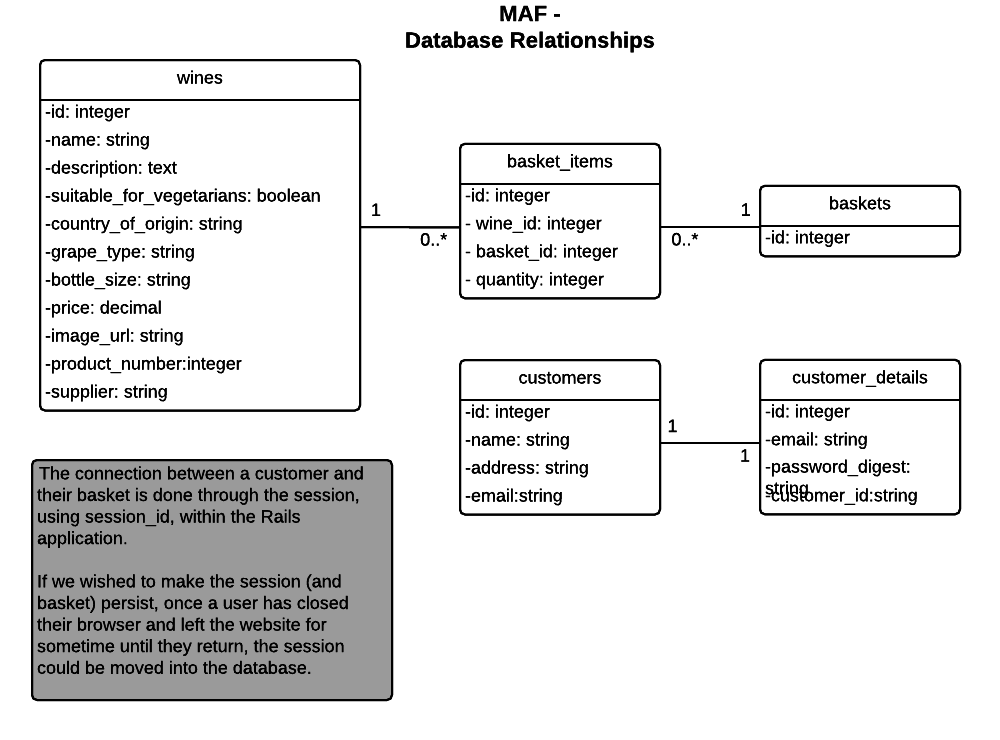
\includegraphics[width=0.5\textwidth]{assets/MAF_Database_relationships}
                \caption{The intended design of the database and relations between tables in the MAF application.}
                \label{fig: Intended MAF Database relationships.} 
\end{figure}


Justify why you built it this way
What is a session? Basket Id and Customer Id for use in login and basket while they are there
How do you get the Wines?
Wines stored with supplier - Supplier in config for if it was deployed, but could also be in Database. Which is better?
Thin Controllers and models - Keep logic seperate, DRY principles?

\subsection{MVC}
\begin{lstlisting}
can have code here
\end{lstlisting}

%----------------------------------------------------------------------------------------
%	WEB SERVICE ARCHITECTURE
%----------------------------------------------------------------------------------------

\section{Web Service Architecure}

Simple web service has two RESTful routes, Orders and Wines. Get Wines with /wines.json, and send Orders with /orders. As RESTful resources, we don't need to direct to a route like 'send\_order' or 'get\_wines'. Just making a GET request on the wines.json returns us the Wines (since last updated, based on headers), and sending a POST to /orders with the json data for a new order automatically routes to 'create' in the Orders controller. Just adds the order as a record into the database.



%----------------------------------------------------------------------------------------
%	TEST STRATEGY
%----------------------------------------------------------------------------------------

\section{Test Strategy}
\subsection{System Testing}
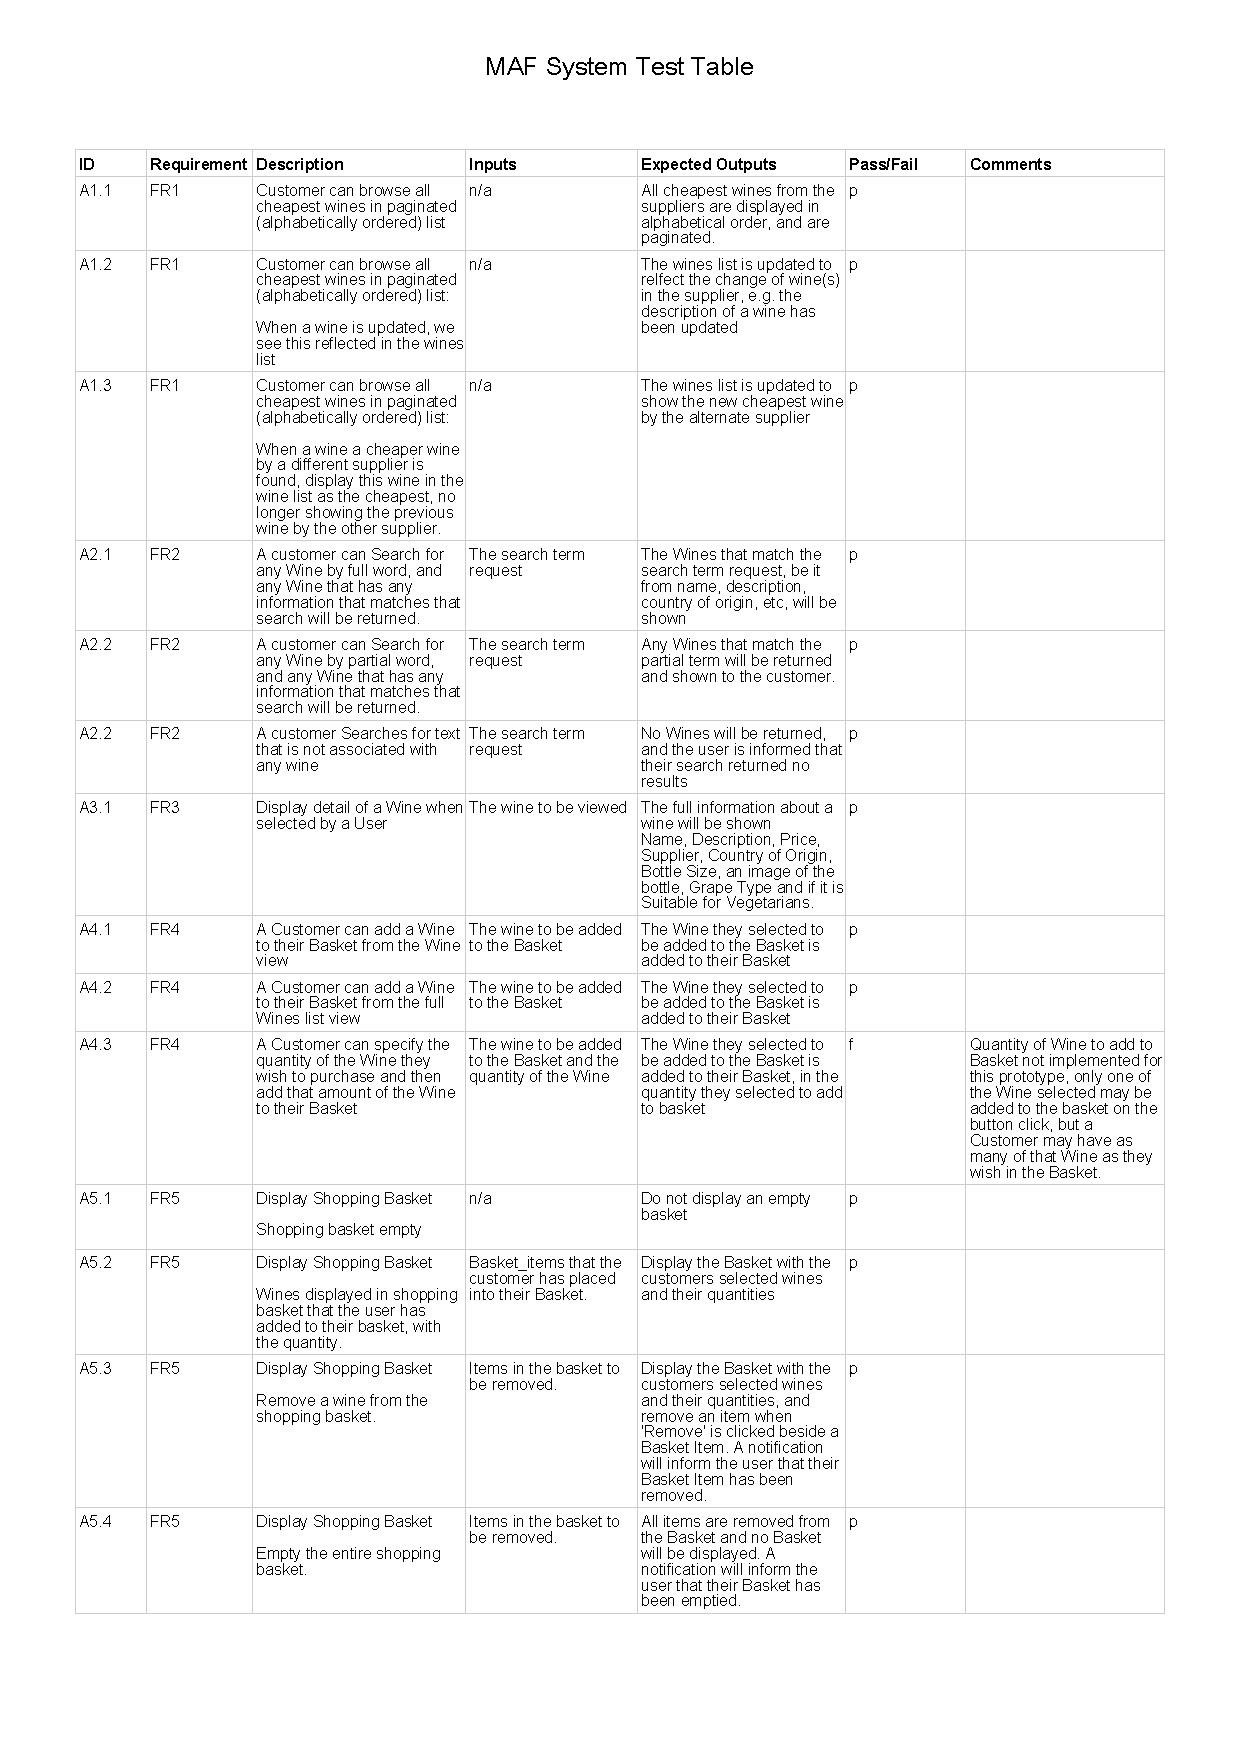
\includepdf[pages=-]{assets/MAF_System_Test_Table.pdf}
\subsection{Unit Test for models and controllers}
Demonstrate implementation of own Unit Tests for models and controllers (show test executions passing, show test names)
Screenshots of tests passing

%----------------------------------------------------------------------------------------
%	SELF-EVALUATION
%----------------------------------------------------------------------------------------

\section{Self-Evaluation}
\subsection{Mark Breakdown}
\subsubsection{Screencast}
Showed 2 Web Service Suppliers running, showed MAF running with all functionality discussed in this report. Expanded on this to show tests passing, Search in depth, etc Showed orders being received by the web suppliers
Mark: /10\%

\subsubsection{Design}
Design diagrams for both how I expected MVC to look and also for my database ideas, along with improvements. Explanation for my designs present and meeting the requirements, backed up through screencast. Documentation quality is okay, could be more in-depth, and design could be improved, but I'm new to Rails and need more experience.
Mark: /20\%

\subsubsection{Implementation: MAF}
Application runs, and meets the requirements (except quantity indicator when adding to basket). Rails controllers make calls to models, and views receive the data from the controllers in order to display it. Code is commented, attributions to code where used and identifier names speak for themselves.
Mark: /25\%

\subsubsection{Implementation: Web Service}
Web Services run, code has comments and names are good. RESTful resources, wines and orders, can call them and the routing sends the request to the controller through the type of request.
Mark: /15\%

\subsubsection{Testing}
Unit tests for each controller, more than just the ones generated by rails, and tests for the models, validations and own methods too. System test table matches assumed customer expectations. Results are discussed and based on these what could be taken forward if this prototype were to be fully implemented
Mark: /15\%

\subsubsection{Evaluation}
Full evaluation of report, MAF and web service, with summary of evaluation below the mark breakdown, with what was learned, difficult and easy.
Mark: /5\%

\subsubsection{Flair}
Implementation of Search using Solr with Sunspot to search partial words from all sections, editing the schema to change the gram of the search. Calling the WebService asynchronously with SuckerPunch, scheduling it to update with rufus-scheduler for hands off updating without interrupting the customer as they browse the website.
Mark: /10\%

\subsubsection{Total}
Mark: /100\%

\subsection{Summary}
I think I met all of the functional requirements as requested (bar quantity indicator in FRwhatever), and the resources as RESTful and data is represented in the Rails way. I know there are areas for improvement (security, clean up, persistent sessions and baskets, better tests, cucumber tests, etc), but as far as the time allowed, my understanding and learning of Rails and this assignment tasking me to just create a prototype, I am happy with the resulting program, and happy I could learn more about Rails and Ruby, how to implement an MVC pattern, talking between web services and even implement external features, like learning configurations of Solr for my search.
I found the most difficult part to be implementing routing, and getting my links in the views to exectue the correct controller actions as I wanted (for the more complex tasks, such as removing the last item from a basket, logging in and sending the webservice order). Before this assignment I had little working knowledge of rails outside of the workshops and a small amount of experience with routing, and doing this assignment helped me get my head around routing and how it works, and has helped me feel comfortable going forward in the future to building more Rails apps when I want to make a web application. 



%----------------------------------------------------------------------------------------
\clearpage

%----------------------------------------------------------------------------------------
%	REFERENCES
%----------------------------------------------------------------------------------------

\begin{thebibliography}{5}

\bibitem{assignment} Chris Loftus, ``MyAlcoholFreeWine.com'',SE31520/CHM5820 Assignment 2015-16, October 27 2015


\end{thebibliography}


\end{document}


